\documentclass[a4paper]{scrartcl}
\usepackage[utf8x]{inputenc}
\usepackage{ucs}
\usepackage{amsmath}
\usepackage{amsfonts}
\usepackage{amssymb}
\usepackage{scrpage2} 
\usepackage{ulem}
\usepackage{tabularx}
\usepackage{cancel}
\usepackage{hyperref}
\usepackage{graphicx}
\usepackage{color}
\usepackage{subfigure}

\newcommand{\imagenumber}[1]{\textcolor{red}{\textbf{#1}}}


\begin{document}
\tableofcontents
\newpage

\section{General Information}
The primary goals of sports biomechanics are to improve athletic performance and to reduce the risk of injury.
In both cases, the underlying problem involves understanding how the human motor system achieves coordinated movement.
Studies of human movement coordination typically involve motion capture (or tracking) in which the movement of markers are tracked in a calibrated space.
The three-dimensional locations of the markers, throughout the movement, can be used to construct a model of the musculoskeletal system.
Many parameters can then be created and used for analyses, but commonly in coordination studies the relative angular displacements, velocities and accelerations between moving segments are used.
Such measures remove the effect of body size and location in the laboratory.
Qualitative techniques such as angle-angle diagrams, phase planes, continuous relative phase, etc. exist, which represent the two-dimensional coupling between various segments, but, unfortunately, are limited to comparisons of two segments at a time.\\
Self-Organizing Maps (SOM\footnote{See \href{http://www.cis.hut.fi/somtoolbox/theory/somalgorithm.shtml}{http://www.cis.hut.fi/somtoolbox/theory/somalgorithm.shtml} for an introduction to SOMs}) have been used as a method for visualizing high-dimensional coordination patterns representing sports techniques.
The advantages associated with SOM analyses are that qualitative changes in coordination patterns may be visualized, the method is objective and thereby helps remove researcher bias, and, is a simpler representation of a complex task which practitioners, coaches, researchers should be able to use.\\
The modules presented in the following provide functionalities that simplify the construction and visualization of self organizing maps based on data from OpenSim\footnote{\href{https://simtk.org/home/opensim}{https://simtk.org/home/opensim}}, a musculoskeletal modeling and simulation software. One module serves as an exporter for data from OpenSim. The second module described in this documentation provides a visualzation for SOMs within OpenSim. It enables the user to display trajectories on top of a umatrix next to a moving 3D model of a human skeleton in a synchronized fashion. This synchronized visualization of the SOM next to the skeleton it corresponds to, enables the user to directly see what change in the trajectory maps to which pose of the body. Therefore the user will probably be able to better understand the SOM and interpret trajectory differences among different athletes.
The process starting with the selection of data in OpenSim and ending with the synchronized visualization of a SOM can be viewed as a chain like sequence of actions.\\
The chain starts with a model in OpenSim that has some movement attached to it. This movement may have been computed by OpenSim using marker data from a 3D tracker but it may also have been acquired in another way.\\
Utilizing the SOM Export module, the user can select data from this movement like joint angles or positions for export to a SOM Toolbox compatible format\footnote{see \cite{toolbox-manual} for a manual of the SOM Toolbox}.\\
In the next step the SOM Toolbox\footnote{see \href{http://www.cis.hut.fi/somtoolbox}{http://www.cis.hut.fi/somtoolbox} for a detailed description} is used to compute a umatrix of the data and save it as \textbf{.cod} file and a \textbf{.data} file.
The \textbf{.cod} file as well as the \textbf{.data} file serve as input for the SOM visualization module.\\
The following sections will give a more detailed description of how the modules extending OpenSim are installed and used.


\section{Installation}
OpenSim is built as a Netbeans Platform application and inherits its the modular design.
Therefore the export module as well as the SOM View module both are deployed as Netbeans Modules (NBM).
In order to install \textbf{.nbm} files in OpenSim, the user has to open the update manager via \textbf{Tools}$\rightarrow$\textbf{Module Manager}.
Now choose \textbf{Install Manually Downloaded Modules (.nbm Files)}, proceed with next and add the respective module files via \textbf{Add...} and again proceed three times with \textbf{Next}.
Now check the checkbox next to the module name and click \textbf{Finish} to conclude the installation process.
The modules are now available via the menu of OpenSim.


\section{Export Module: OpenSim to SOM Toolbox}
In order to train SOMs with data from OpenSim, some kind of export function for data in OpenSim to a format that can serve as input for the SOM toolbox is required. The module described in this section provides this feature and gives the user some options on what he wants to export in what way.
It exports properties of a model that are changed by a motion over time. The user can choose the properties and the time interval at which they will be exported.
\subsection{Usage}
Before you can export data to SOM Toolbox you first need to load a model and at least one suitable motion into OpenSim.
Assuming you have already installed the export module in OpenSim, you can find the export dialog via \textbf{File}$\rightarrow$\textbf{Export to Matlab SOM}.
\begin{figure}
\label{fig:som-export}
\centering
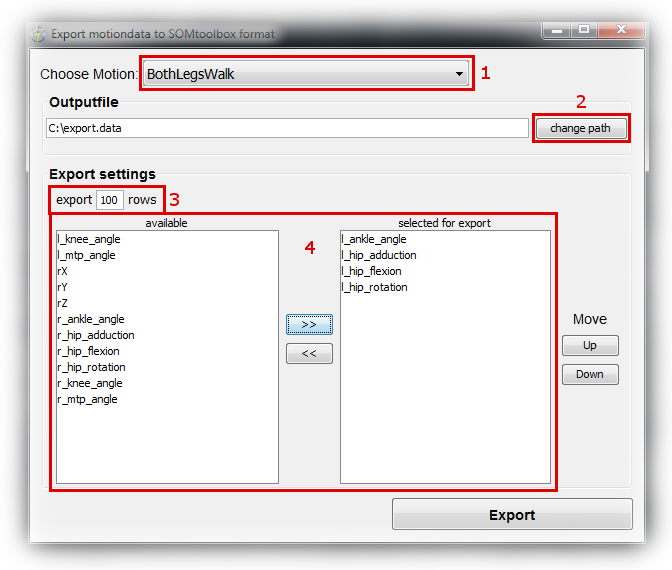
\includegraphics[width=10cm]{graphics/screen_exporter_1.png}
\caption{Screenshot of the export dialog}
\end{figure}
It is depicted in figure \ref{fig:som-export}. The red frames and numbers are not part of the screenshot but will simplify the description of export settings that you can adjust. \\
The export dialog will always export data from the current model. You can change the current model by \textbf{right clicking} on a model in the \textbf{Navigator} panel of OpenSim and choosing \textbf{make current}.\\
Right after the export dialog has popped up, you should make sure that the correct motion is selected in case there is more than one loaded motion for the current model. The listbox referred to as \imagenumber{1} in figure \ref{fig:som-export} contains all motions that are available in the current model. Choose the motion you want to export from.\\
You can specify the location where the data will be saved either by clicking the \textbf{change path} button (\imagenumber{2}) and selecting a filename in the dialog that shows up or directly by writing a path in the textfield next to the button.\\
Through the field marked as \imagenumber{3} in the picture you can set the number of samples (rows) that will be exported from the motion.
Motions are represented in OpenSim by a set of fixed states at certain points in time. OpenSim will interpolate between these states as data between these points in time is requested. This enables the user to select arbitrary many samples for export.\\
The frame denoted by \imagenumber{4} covers two list boxes and 2 buttons between them.
The listbox on the left side initially contains all properties of the model that are affected by the currently selected motion (\imagenumber{1}). You can mark properties (single or multiple) for export by selecting them in the left listbox and clicking the $>>$ button. The respective entries will appear in the right listbox which contains all entries that will be exported. If you want to change the export order of the entries, you can do so by selecting one or multiple entries in the right listbox and clicking either the \textbf{up} or \textbf{down} button to move them.\\
Finally, click the \textbf{export} button in the lower right corner of the window to perform the export process.
In case you want to export data from multiple motions to one file, simply choose the same file as destination for all the motions. When you are asked if you want to append or overwrite, answer append. The exported trials will be identified by the name of their OpenSim motion. Note that if you output multiple motions to the same file the number and order of the columns has to stay the same.


\section{Processing the data with the SOM Toolkit}
\label{sec:som-toolkit}
%Drauf hinweisen, dass das Programm momentan nur hexagonale umatrices kann

\section{SOM View Module}
%TODO noch erwähnen, dass man das fenster über "windows"->SOMView aufruft
With the SOM View module OpenSim is extended by a visualization for SOMs. You can display the umatrix in several different ways. Trajectories for multiple trials can be drawn on top of the umatrix. The view module has its own window which is meant to be placed next to OpenSim or even on another screen. Figure \ref{fig:som-view} shows a screenshot of the window. The left side of the window contains control elements, the right side displays the actual umatrix and trajectories. As a model that is loaded in OpenSim performs a motion in the OpenSim 3D view, trajectories corresponding to motions of this model can build up in the SOM visualization window in a synchronized fashion. The speed and progress of both, the motion in OpenSim and the trajectories in the SOM Viewer are controlled via the OpenSim motion control elements as shown in figure \ref{fig:opensim-motion-control}. Seeing a moving skeleton and trajectories that build up on top of umatrix at the same time offers the opportunity to relate skeleton poses to trajectory states.
\begin{figure}
\centering
\subfigure[SOM View window]{
	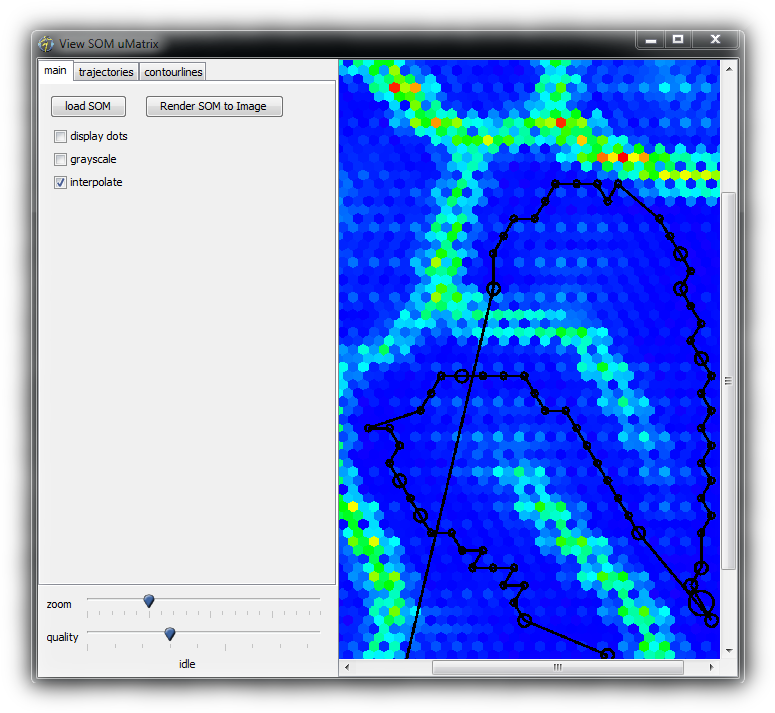
\includegraphics[width=9cm]{graphics/somview_screenshot.png}
	\label{fig:som-view}
	}
\subfigure[OpenSim motion controls]{
	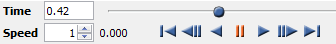
\includegraphics[width=9cm]{graphics/somview_motion_controls.png}
	\label{fig:opensim-motion-control}
	}
\caption{Screenshots of SOM View window and OpenSim motion controls}
\label{fig:som-view-and-mot-controls}
\end{figure}

\subsection{Usage}
The user interface of the SOM visualization window is split into two major parts. The left part contains controls for the visualization which is located in the right part of the window. The controls are further topically divided in 3 tabs.
Three elements are present in all the tabs. One slider to zoom in the umatrix display (\imagenumber{1}), another slider to adjust the rendering quality (\imagenumber{2}) and a field displaying status messages (\imagenumber{3}).
Usually the quality that is set by default is sufficient. If you should need to take a very close look at the umatrix or want to export it in high quality you can increase the image resolution with this slider. Since the memory that OpenSim can use is quite scarce you might need to increase its maximal heap size. See \ref{sec:max-heap-size} for a detailed description.
In the following, the functions offered by the SOM View module will be described in greater detail.

\subsubsection{Main Controls}
\begin{figure}
\centering
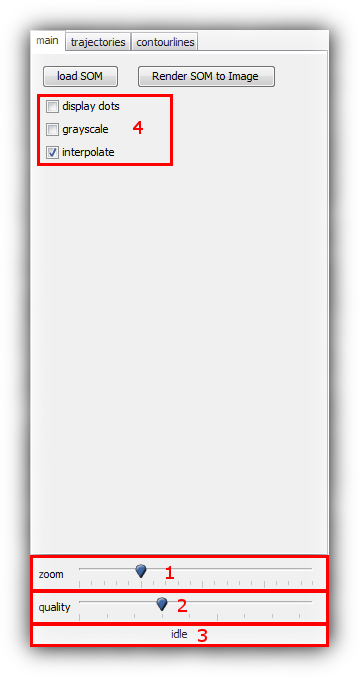
\includegraphics[width=4cm]{graphics/somview_main.png}
\caption{SOM View - main controls}
\label{fig:controls-main}
\end{figure}
Before you can tweak around with the settings and controls in the SOM View window you first need to load a umatrix. If you want to display trajectories you need to load them as well. See section \ref{sec:trajectories} on how to do that.
The umatrix can be loaded from \textbf{.cod} format file as specified in \cite{toolbox-manual}. See section \ref{sec:som-toolkit} on how to create \textbf{.cod} and \textbf{.data} files.
By clicking the \textbf{load SOM} button as shown in the upper left corner of figure \ref{fig:controls-main} and selecting the respective \textbf{.cod} file in the file open dialog, you can load a umatrix. After you have done so, you will see a grey version of a umatrix in the display area in the right half of the window. You can change the appearence of the umatrix with the controls as denoted by \imagenumber{4} in figure \ref{fig:controls-main}.
Your options are displaying the umatrix in a greyscale version, a coloured version and in a version where the color of the nodes themselves is interpolated between the hexagons around them.
Via the \textbf{Render SOM to Image} button in the upper right corner of the main control tab you can export an image of the umatrix that is currently displayed. Consider increasing the quality with the quality slider for export.

\subsubsection{Trajectories}
\label{sec:trajectories}

\begin{figure}
\begin{center}
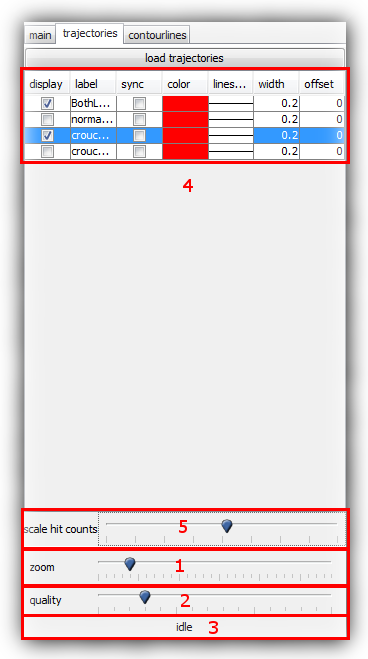
\includegraphics[width=4cm]{graphics/somview_trajectories.png}
\end{center}
\caption{SOM View - trajectory controls}
\label{fig:controls-trajectories}
\end{figure}
The trajectory tab of the SOM View window offers several elements that let you load and customize trajectories.
At first you need to load trajectories from file using the file open dialog that pops up if you click the \textbf{Load trajectories} button at the top of the trajectory control panel. The file has to be in the \textbf{.data} format as defined in \cite{toolbox-manual}.
After the trajectories have been processed (which may take a while) they are displayed in a row wise fashion in the table marked as \imagenumber{4}. 
The trajectories are identified by the label that is read from the \textbf{.data} file.
You can adjust several properties for each trajectory individually
\begin{itemize}
    \item \textbf{display}: Turns drawing the trajectory on top of the umatrix on and off
    \item \textbf{sync}: Turns the synchronization with the model motions in OpenSim on and off
    \item \textbf{color}: Color of the trajectory
    \item \textbf{linestyle}: line style the trajectory will be drawn with (e.g. dotted line)
    \item \textbf{thickness}: thickness of the trajectory line
	\item \textbf{offset}: offset from the node center $\rightarrow$ reduces overlapping when multiple trajectories are drawn
\end{itemize}
Hexagons along the trajectory path can more than once be BMUs. In order to indicate how often they were hit, circles with varying size are drawn ontop of the hexagons. The bigger the circle is, the more often this hexagon was a best matching unit (BMU). You can adjust the overall scaling of those circles with the slider marked as \imagenumber{5} in figure \ref{fig:controls-trajectories}.

\subsubsection{Contour lines}
\begin{figure}
\begin{center}
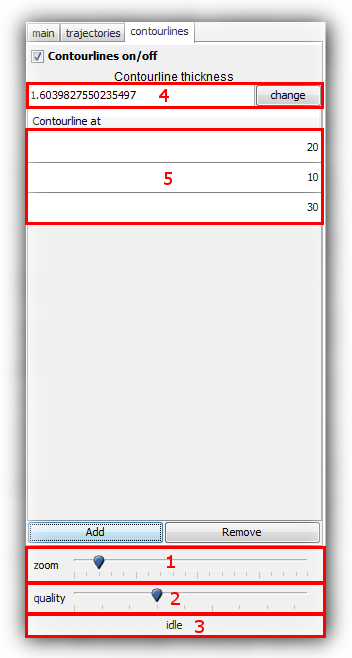
\includegraphics[width=4cm]{graphics/somview_contourlines.png}
\end{center}
\caption{SOM View - contour line controls}
\label{fig:controls-trajectories}
\end{figure}
To get a better understanding of the value differences in the umatrix, you can display contour lines on a smoothed version of the umatrix. If you imagine the umatrix as some kind of topographic map you might find those contour lines familiar.
You can add and remove lines by clicking the \textbf{Add} and \textbf{Remove} buttons on the bottom of the contour line control panel as shown in figure \ref{fig:controls-trajectories}.
Each line is specified by a ``height'' value. Every pixel in the umatrix image is drawn in black if it has the specific value that you specified for a contour line. This way, continuous lines appear on the umatrix that indicate certain heights in the topography. The contours are usually not equally thick at every position of the line. If the line is thick, that means that the slope is small at this part of the map, if it is thin there is a huge slope. An image of the control panel where three contour lines are specified can be seen in figure \ref{fig:controls-trajectories} as \imagenumber{5}.
You can adjust the base thickness of the lines by changing the value in the textbox marked as \imagenumber{4}.

\section{Problem - Solution}
There are some known issues that stem from the fact, that we only provide a module for OpenSim and are therefore bound to some limits that come with OpenSim. If you should encounter any problems during the use of these modules, this is the section to read.
\subsection{Increasing max heap size}
\label{sec:max-heap-size}
In case you want to view or export high resolution versions of the umatrix and trajectory images created with the SOM View module, an error might occur saying \\ 
\textit{java.lang.OutOfMemoryError: Java heap space}. This is due to the fact that OpenSim (current version 2.4.0) by default only uses up to 64 MB of heap space. You can increase this space by modifying the file \verb|opensim.conf| that is located in the \verb|etc| folder of your OpenSim installation directory (example: \verb|C:\OpenSim2.4.0\etc\opensim.conf|).
This file contains a line starting with \verb|default_options=| followed by some command line arguments that are framed by quotation marks.
Changing the default command line arguments \verb|-J-Xms24m -J-Xmx64m| to \verb|-J-Xms256m -J-Xmx512m| and restarting OpenSim will solve your memory problem.
\subsection{Red ball issue in OpenSim}
During the development of the SOM View and the export module a problem with the 3D view of a model in OpenSim came up that is not related to the modules presented in this documentation. However, since there is an easy solution it will be covered here as well. If you install OpenSim on non-US copies of windows, sometimes the models loaded in OpenSim appear as a big red ball instead of e.g. bones and  muscles. You can resolve this issue by modifying the configuration file that was described in \ref{sec:max-heap-size} (example path: \verb|C:\OpenSim2.4.0\etc\opensim.conf|).
You have to modify an option specified in the \verb|default_options=| line. Change the \verb|-J-Duser.language=| argument to \verb|en| resulting in \verb|-J-Duser.language=en|. Restart OpenSim and the problem should be resolved.

\bibliography{user_documentation}
\bibliographystyle{alpha}

\end{document}